\chapter{Uvod}
    Projekt FERSAT, koji se od 2018. godine provodi na Fakultetu elektrotehnike i računarstva, uključuje izradu i lansiranje CubeSat satelita te korištenje satelita u svrhu prikupljanja informacija o svjetlosnom zagađenju i debljini ozonskog omotača. Satelit u izradi dimenzija je približno 10 cm x 10 cm x 10 cm, volumena jedne litre i ne teži od 4/3 kilograma, što ga svrstava u skupinu satelita formata CubeSat 1U \cite{fersat_stranica_projekta}. Očekivani životni vijek satelita je 3 godine, a bit će postavljen u Zemljinoj orbiti na visini između 500 i 600 kilometara. Slika \ref{fig:fersat} prikazuje izgled planiranog satelita.
    
    \begin{figure}[htb]
        \centering
        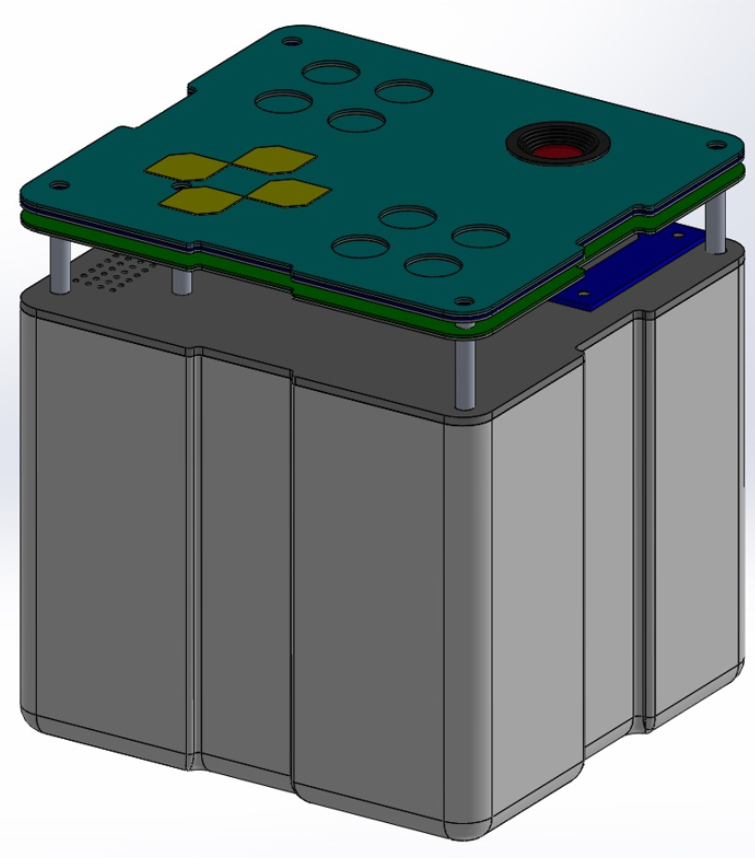
\includegraphics[height=7cm]{slike/fersat.png}
        \caption{Skica planiranog izgleda FERSAT-a. Prikazani su korisni teret \engl{payload} i platforma \engl{bus}. \cite{fersat_stranica_projekta}}
        \label{fig:fersat}
    \end{figure}
    
    Planirani korisni teret \engl{payload} FERSAT-a podijeljen je na tri podsustava:

    \begin{itemize}
        \item kamera za snimanje površine Zemlje i zemaljskog horizonta,
        \item detektori svjetla u vidljivom i ultraljubičastom dijelu spektra za mjerenje svjetlosnog onečišćenja i debljine stupca ozona,
        \item komunikacijski sustav u radijskom X-pojasu (10.45 GHz) za prijenos podataka na Zemlju.
    \end{itemize}

    Radom korisnog tereta upravlja \textit{Payload Data Handler} (PDH) računalo. Zadaća je PDH računala prikupiti podatke iz senzorskog podsustava i kamere, pohraniti ih u trajnu memoriju \engl{non-volatile memory} te poslati prikupljene podatke na Zemlju korištenjem komunikacijskog podsustava. Kao PDH računalo odabran je mikrokontroler STM32L471VGT6 proizvođača ST Microelectronics.

    Za rad ostalih podsustava satelita koji nisu direktno vezani uz koristan teret (npr. upravljanje položajem satelita, slanje telemetrijskih podataka na Zemlju) brine se \textit{Command and Data Handler} (CDH) računalo. CDH računalo također upravlja napajanjem korisnog tereta i šalje naredbe PDH računalu. Komunikacija CDH i PDH računala odvija se korištenjem sučelja CAN (\textit{Controller Area Network}). Konkretno CDH računalo u trenutku pisanja ovog teksta još nije odabrano.

    Slika \ref{fig:fersat_blok} prikazuje blok dijagram cijelog sustava. U okviru ovog rada razvijena je programska potpora PDH računala za prikupljanje i obradu podataka senzorskog podsustava.
    
    \begin{figure}[htb]
        \centering
        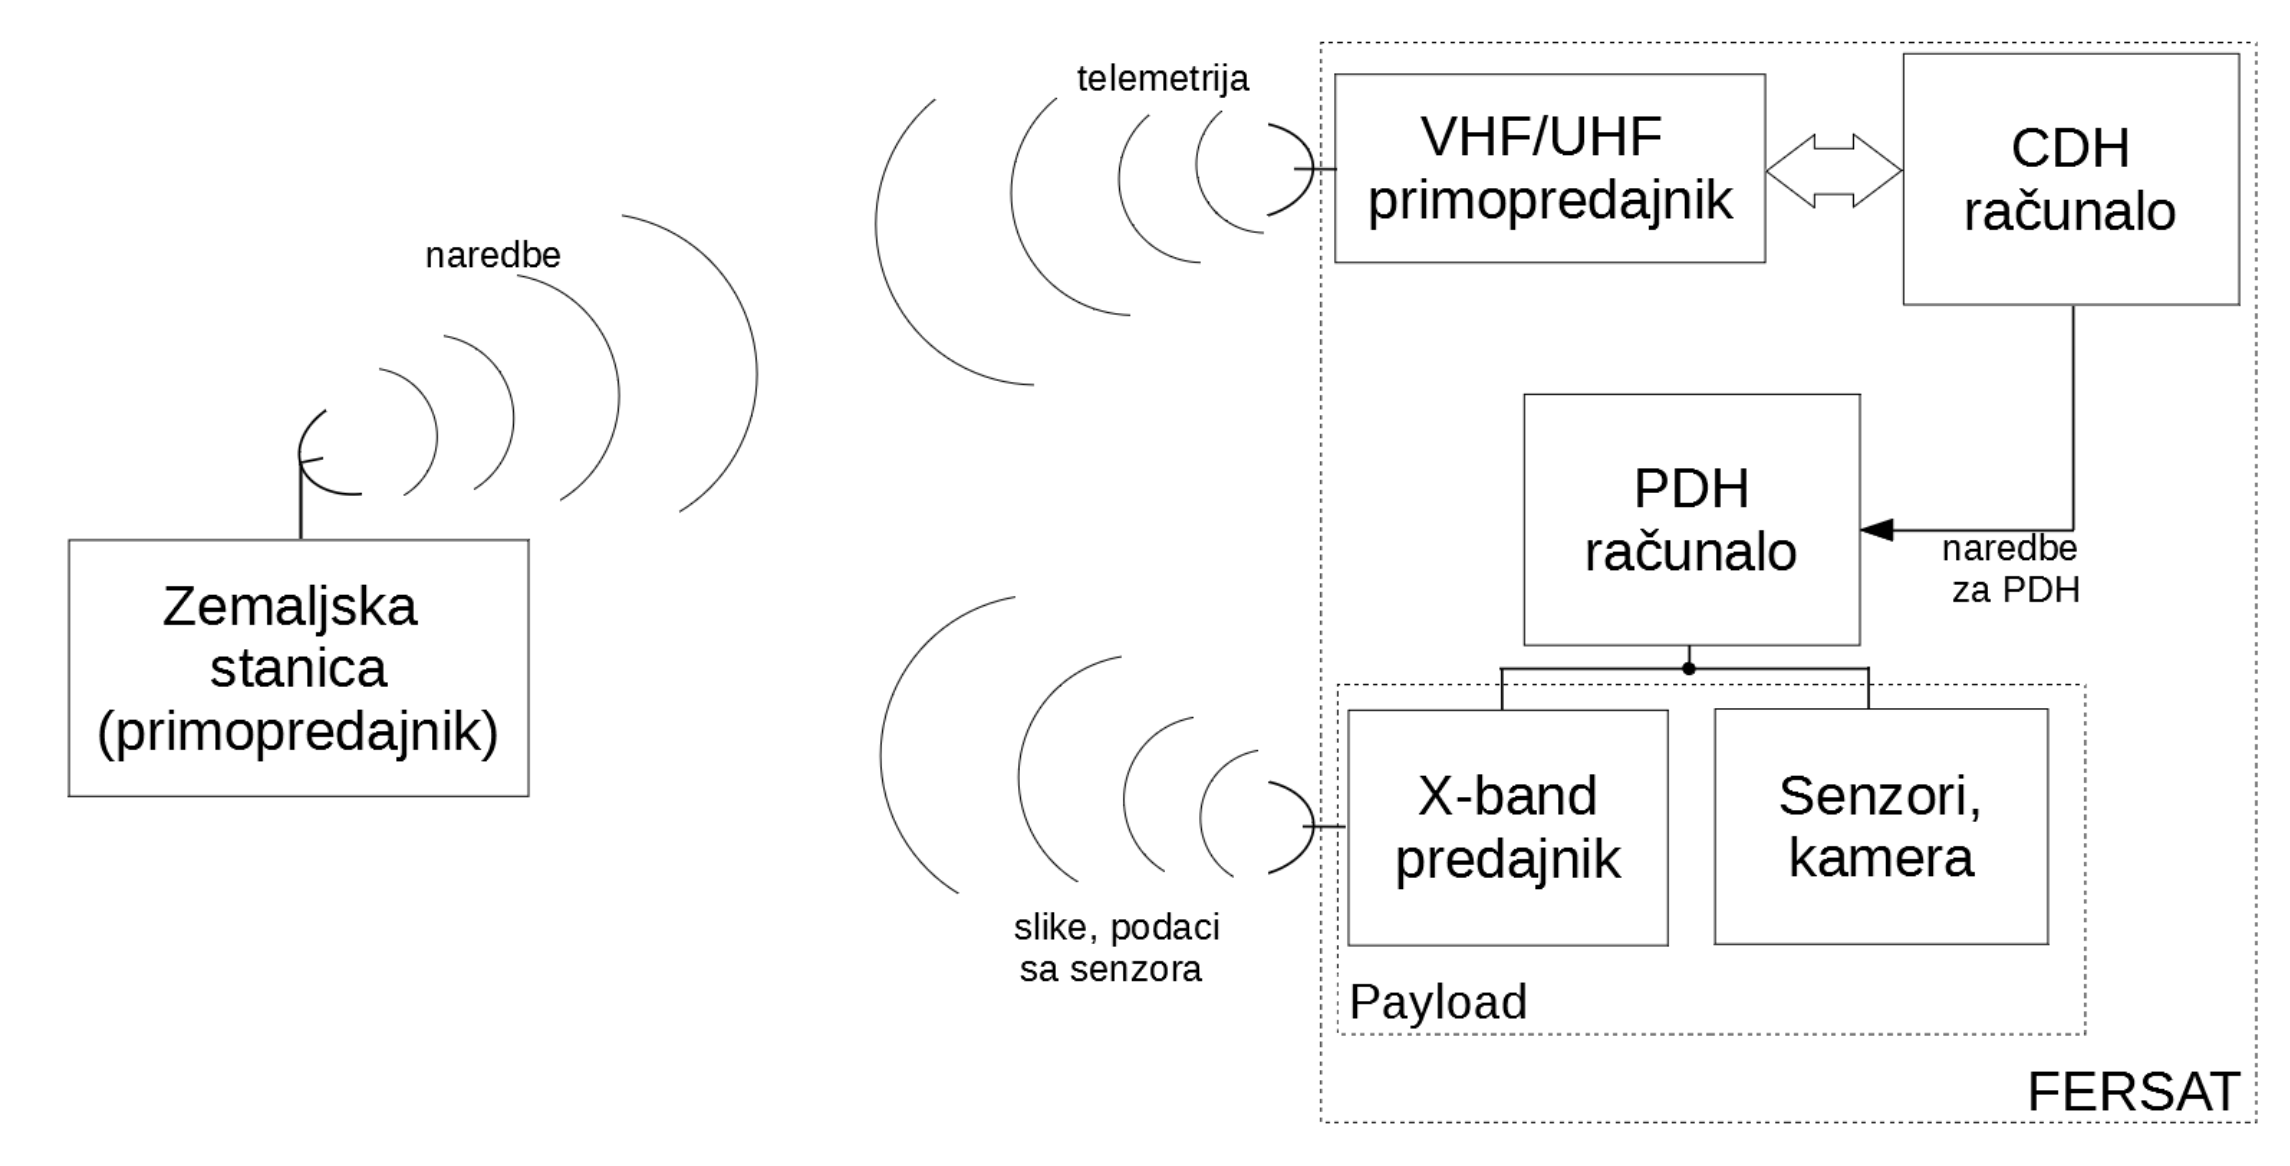
\includegraphics[width=\textwidth]{slike/fersat_blok_dijagram.png}
        \caption{Blok dijagram FERSAT-a i komunikacija sa zemaljskom postajom \cite{diplomski_goran_petrak}}
        \label{fig:fersat_blok}
    \end{figure}

    Senzorski podsustav ima dvije temeljne zadaće. Prva od njih je korištenjem fotosenzora koji rade u vidljivom dijelu elektromagnetskog spektra prikupiti podatke na temelju kojih će biti moguće odrediti udio LED rasvjete u naseljenim mjestima u odnosu na konvencionalnu natrijevu, metal-halidnu i fluorescentnu javnu rasvjetu. Razvijen je algoritam koji na temelju obrade signala multispektralnog svjetla sa Zemlje može odrediti ovu informaciju \cite{diplomski_jakov_tutavac}. Mjerenje udjela LED rasvjete zanimljivo je zbog mogućih negativnih utjecaja plavog svjetla na ljudsko zravlje, kojeg LED rasvjeta emitira u znatno većem intenzitetu nego konvencionalna \cite{falchi_light_pollution}.

    Druga je zadaća senzorskog podsustava mjerenje propusnosti i refleksije atmosfere za ultraljubičasto svjetlo u svrhu određivanja debljine ozonskog omotača. Za mjerenje se koriste PureB detektori ultraljubičastog zračenja razvijeni na FER-u \cite{diplomski_filip_bogdanovic} i algoritmi razvijeni za tu namjenu \cite{zavrsni_kristian_stepancic}. Uspješna mjerenja po prvi put bi potvrdila mogućnost korištenja ove tehnologije u mjerenjima debljine ozonskog omotača iz svemira.

    Upravljačko sklopovlje potrebno za rad PDH računala već je razvijeno \cite{zavrsni_filip_juric}. Tiskana pločica PDH računala, osim mikrokontrolera STM32L471VGT6, sadrži i vanjsku \textit{Flash} memoriju, sustav za napajanje, sklop za kontrolu izvođenja programa \engl{watchdog}, upravljački sklop za CAN komunikaciju i konektore za povezivanje s ostalim dijelovima sustava. PDH pločica bit će smještena ispod senzorske pločice, u takozvanoj \textit{stack-up} konfiguraciji (slika \ref{fig:fersat_3d}).

    \begin{figure}[htb]
        \centering
        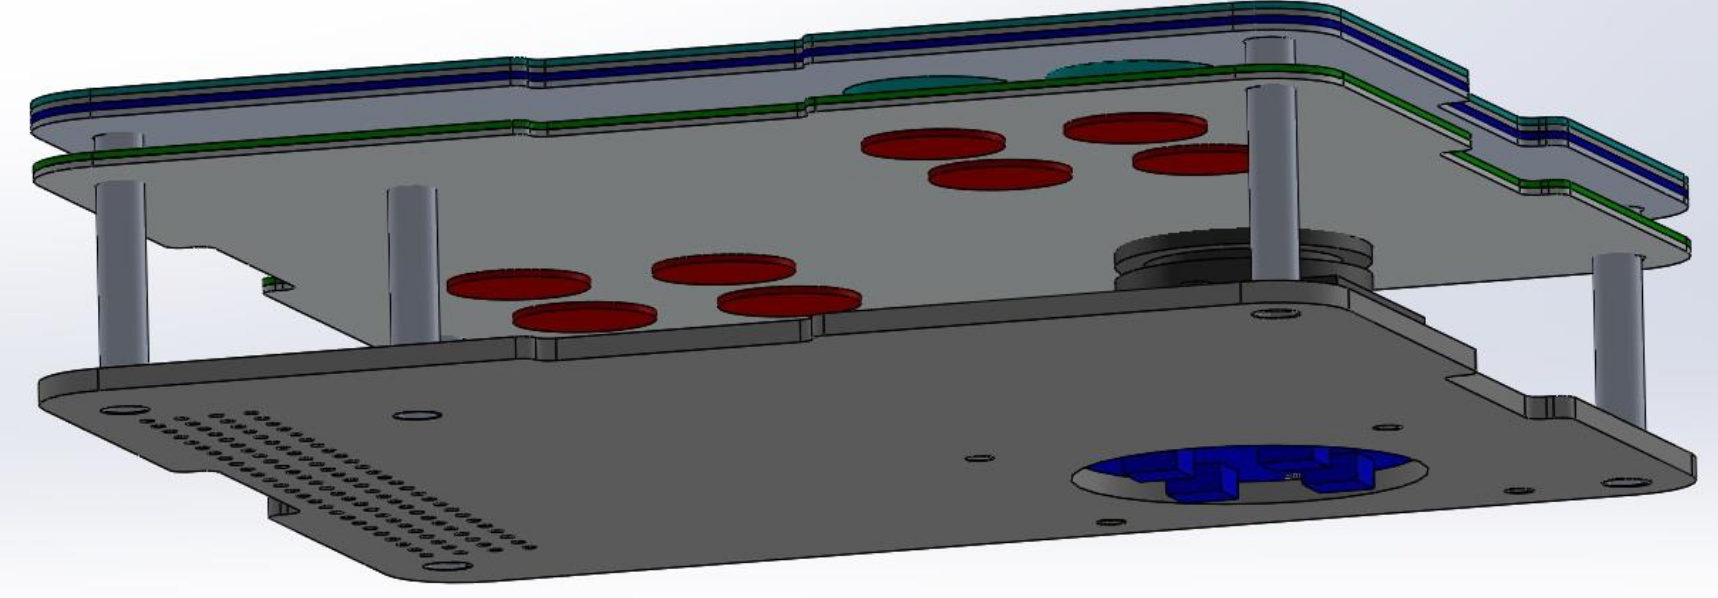
\includegraphics[width=\textwidth]{slike/fersat_3d.png}
        \caption{Trodimenzionalni model korisnog tereta FERSAT-a. PDH računalo smješteno je na donjoj pločici, a senzorski podsustav na srednjoj \cite{zavrsni_filip_juric}.}
        \label{fig:fersat_3d}
    \end{figure}

    Također, u sklopu projekta FERSAT razvijen je i dio programske potpore PDH računala \cite{diplomski_goran_petrak}. No, kako je u međuvremenu došlo do promjene izbora mikrokontrolera PDH računala i promjene dijela sklopovlja senzorskog podsustava, dijelove te programske potpore bilo je potrebno prilagoditi ili ponovno razviti.
    
    Nastavak rada strukturiran je na sljedeći način. U poglavlju 2 opisano je komunikacijsko sučelje između mikrokontrolera STM32L471VGT6 i senzorskog podsustava (SPI - \textit{Serial Peripheral Interface}). Detaljan opis sklopovlja senzorskog podsustava dan je u poglavlju 3. U poglavlju 4 opisani su razvijeni upravljački programi za pojedine sklopovske komponente, cjelokupna programska potpora za senzorski podsustav, i integracija s ostalim dijelovima programske potpore PDH računala korištenjem operacijskog sustava za rad u stvarnom vremenu FreeRTOS.
